\subsection{Top quarks}

At the LHC energies, the dominant production channel for top quark pairs is 
gluon-gluon fusion which is responsible for 80--95\% of the total top pair production. 
The remaining $\mathrm{t}\bar{\mathrm{t}}$ pairs are from quark-antiquark annihilation. 

As discussed in Ref.~\cite{d'Enterria:2015jna}, top measurements probe the 
nuclear gluon density in an unexplored kinematic regime around Bjorken-$x$ 
values, $x \sim 2m_{\mathrm{t}}/\rootsNN \sim 5 \cdot 10^{-3}-0.05$, 
and virtualities $Q^{2} \sim m_{\mathrm{t}}^{2} \sim 3 \cdot 10^{4}$ GeV, 
a region characterized by anti-shadowing corrections. High accuracy measurements 
of the perturbative $\mathrm{t}\bar{\mathrm{t}}$ cross section in pp collisions, 
have provided a strong constraint on existing NNLO PDF sets, in particular on 
the large-$x$ gluon PDF~\cite{Czakon:2013tha}. A measurement of the 
$\mathrm{t}\bar{\mathrm{t}}$ cross section as function of pseudorapidity 
in pPb collisions will constrain the modification of nuclear gluon PDF in 
an $x$ range that is currently unconstrained. The top quark cross section 
is expected to increase at midrapidity due to anti-shadowing effect,
while at backward rapidities ($\eta_{t}<-1.5$) large-$x$ region is reached 
and the EMC effect takes over~\cite{d'Enterria:2015jna}.

\begin{figure}[h!]
\begin{center}
  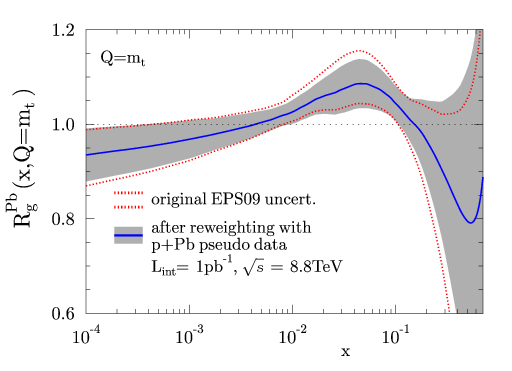
\includegraphics[width= 0.47\textwidth]{figures/top/gluons2.png}
  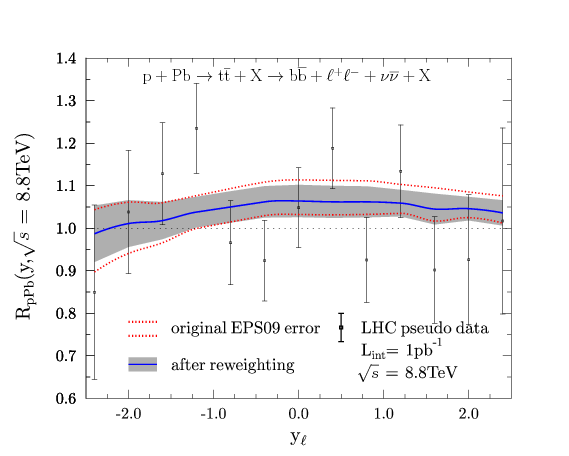
\includegraphics[width= 0.47\textwidth]{figures/top/data2.png}
  \caption{Estimated impact on the nuclear gluon distribution function
   from nuclear modification factor measurement of $\mathrm{t}\bar{\mathrm{t}}$ 
   decay leptons in pPb collisions at \rootsNN\ = 8.16 TeV.
  Figures are taken from Ref.~\cite{d'Enterria:2015jna}.
  }
\label{fig:ttnPDF}
\end{center}
\end{figure}

Figure~\ref{fig:ttPPbProjections} shows the expected number of 
$\mathrm{t}\bar{\mathrm{t}}$ pairs (left panel) and corresponding 
statistical uncertainty (right panel) as function of total integrated 
luminosity. The total number of top pairs is calculated as follows:
\begin{equation}
N_{\mathrm{t}\bar{\mathrm{t}}} = \sigma_{\mathrm{t}\bar{\mathrm{t}}} \cdot A \cdot \mathcal{B} \cdot \mathcal{L}_{\mathrm{int}} \cdot \mathcal{A} \cdot \epsilon,
\end{equation}

\noindent with $\sigma_{\mathrm{t}\bar{\mathrm{t}}}=244$~pb$^{-1}$ 
corresponding to the measurement in 8 TeV pp collisions~\cite{Khachatryan:2016mqs}, 
$A$ the mass number of lead (208), $\mathcal{B}$ the branching ratio 
of the selected final state, $\mathcal{L}_{\mathrm{int}}$ the total integrated luminosity, 
$\mathcal{A}$ the fraction of events within the CMS acceptance and 
$\epsilon$ the typical reconstruction efficiency in the CMS detector.
The desired integrated luminosity for making a $\mathrm{t}\bar{\mathrm{t}}$
cross section measurement in pPb collisions at \rootsNN\ = 8 TeV is 200--100 nb$^{-1}$,
which gives a statistical uncertainty of 10--14\%. Such a goal is feasible to
achieve in the 2016 pPb run.

\begin{figure}[h!]
\begin{center}
  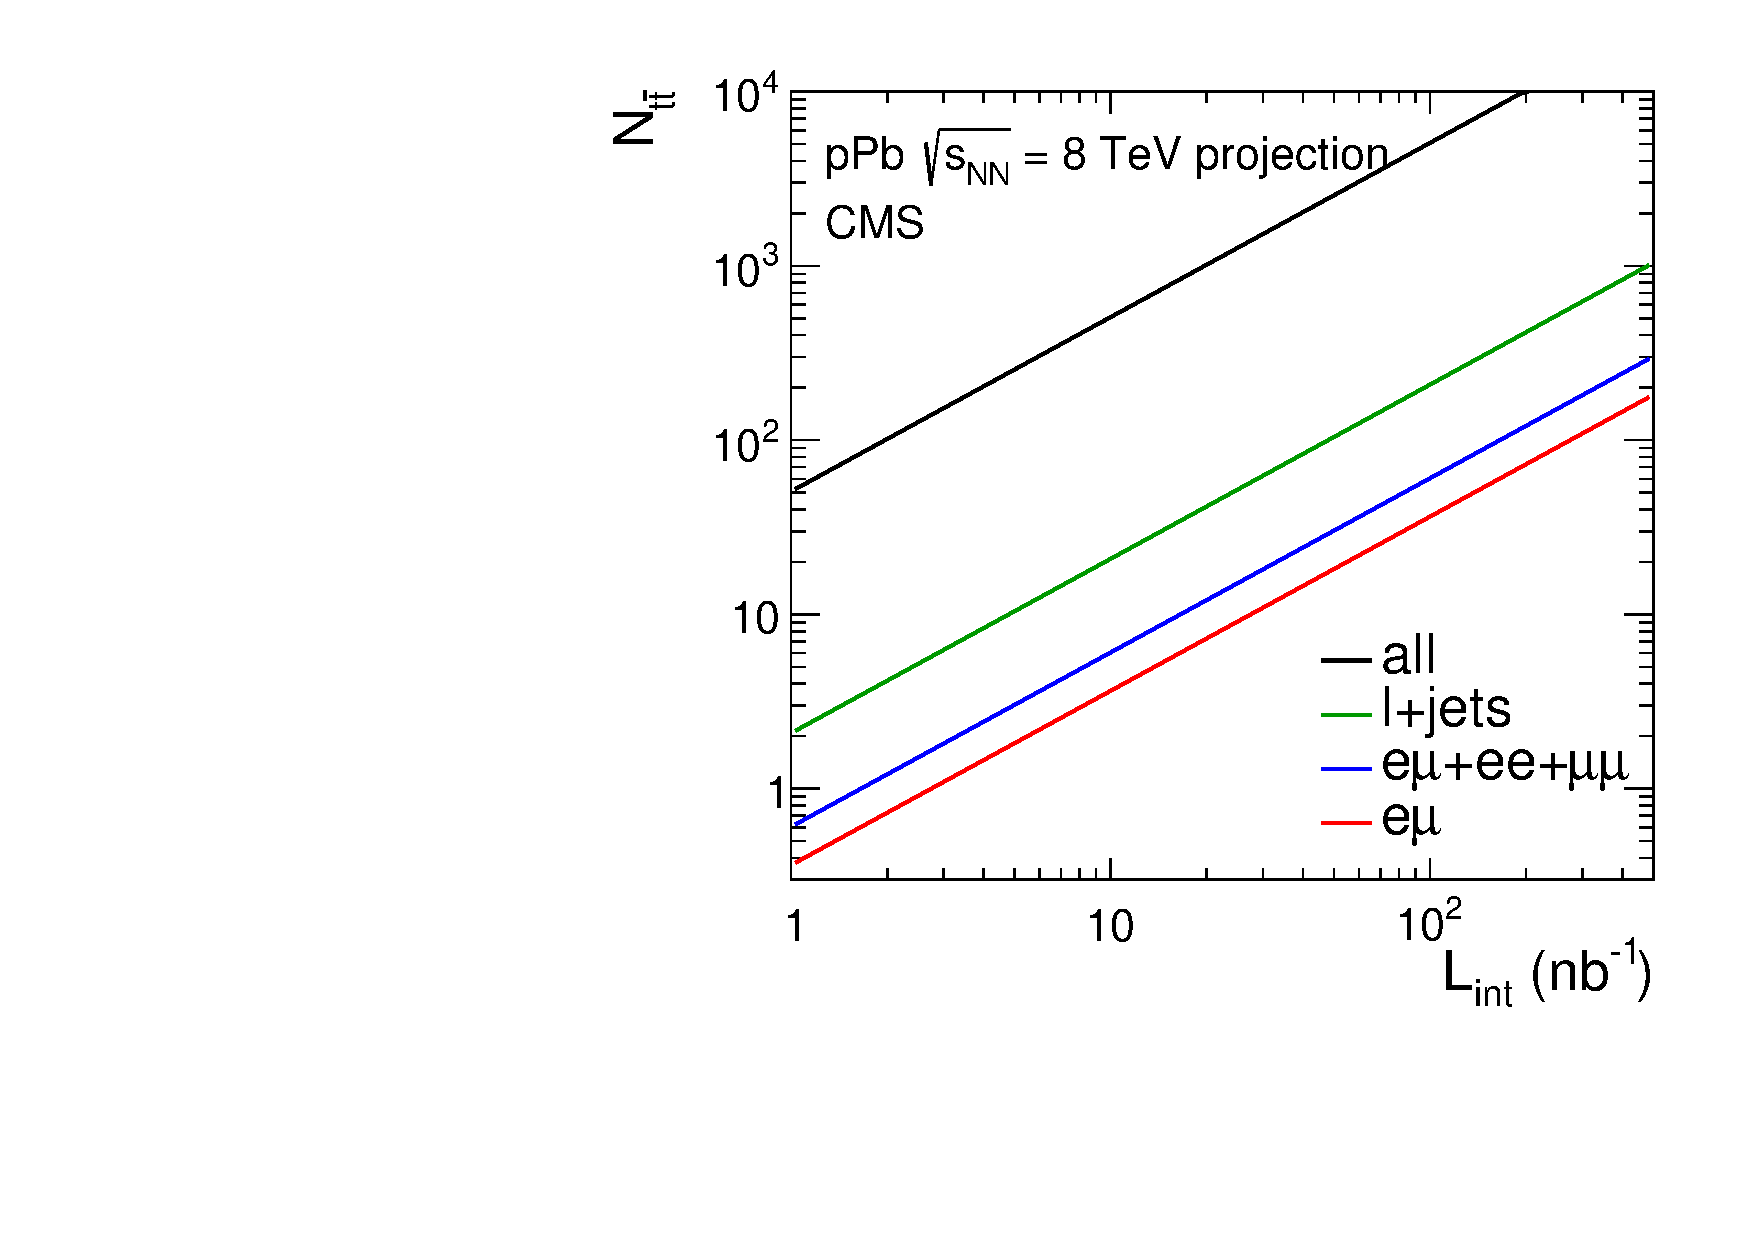
\includegraphics[width= 0.47\textwidth]{figures/top/ProjectedTTbarYield.pdf}
  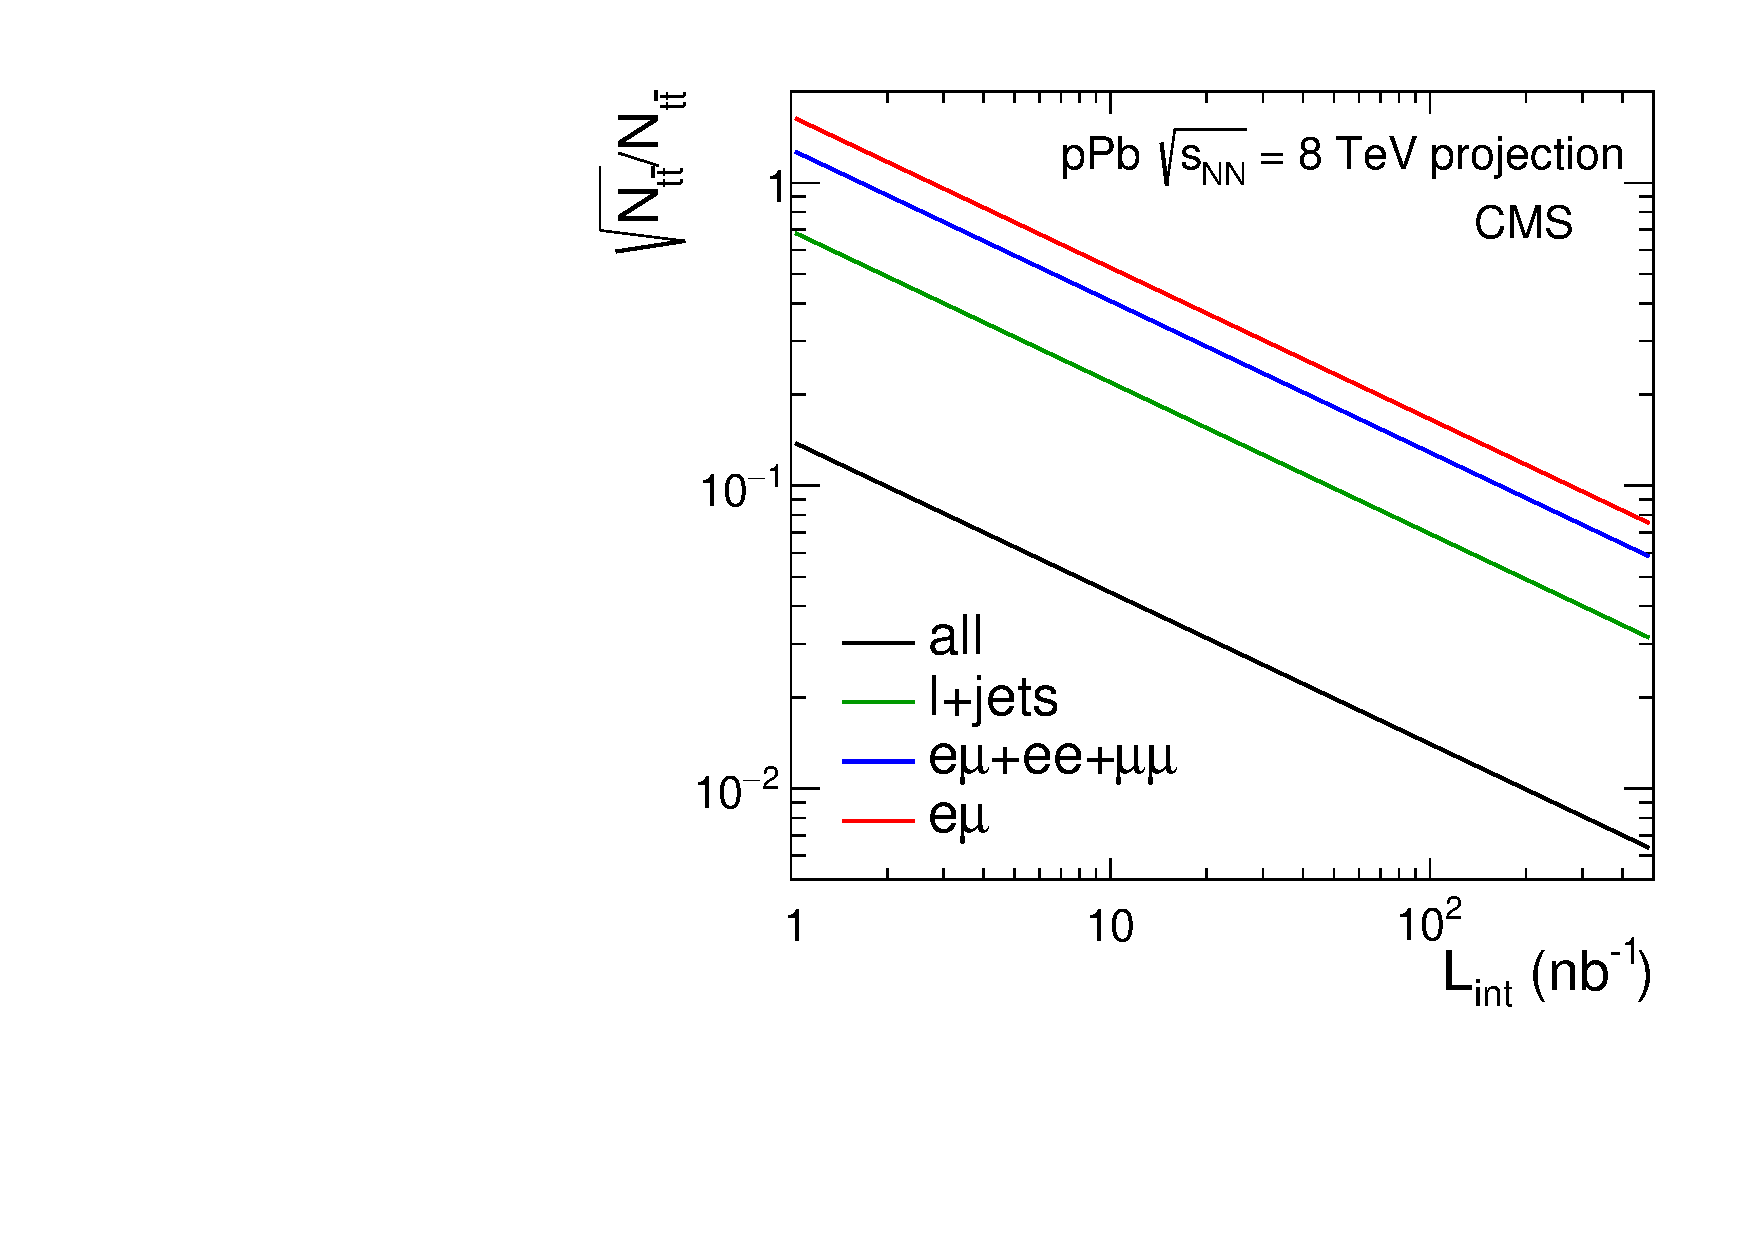
\includegraphics[width= 0.47\textwidth]{figures/top/ProjectedTTbarStatUnc.pdf}
  \caption{Left panel: Expected number of $\mathrm{t}\bar{\mathrm{t}}$ events 
  for several channels in pPb collisions at \rootsNN\ = 8.16 TeV as a function 
  of total integrated luminosity. Right panel: Corresponding statistical uncertainty 
  as a function of total integrated luminosity.
  }
\label{fig:ttPPbProjections}
\end{center}
\end{figure}

The jet energy scale, Drell-Yan ($DY$) and $W$+jets physics signal subtraction 
are the dominant systematic uncertainties for the $\mathrm{t}\bar{\mathrm{t}}$ 
cross section measurements. All these uncertainties can be reduced by measuring 
them directly in the data, which is only possible with a large integrated luminosity. 
The evolution of the systematic and statistical uncertainty as function of total 
integrated luminosity in various pp measurements at CMS is shown in Fig.~\ref{fig:ttStatSyst}.

\begin{figure}[h!]
\begin{center}
  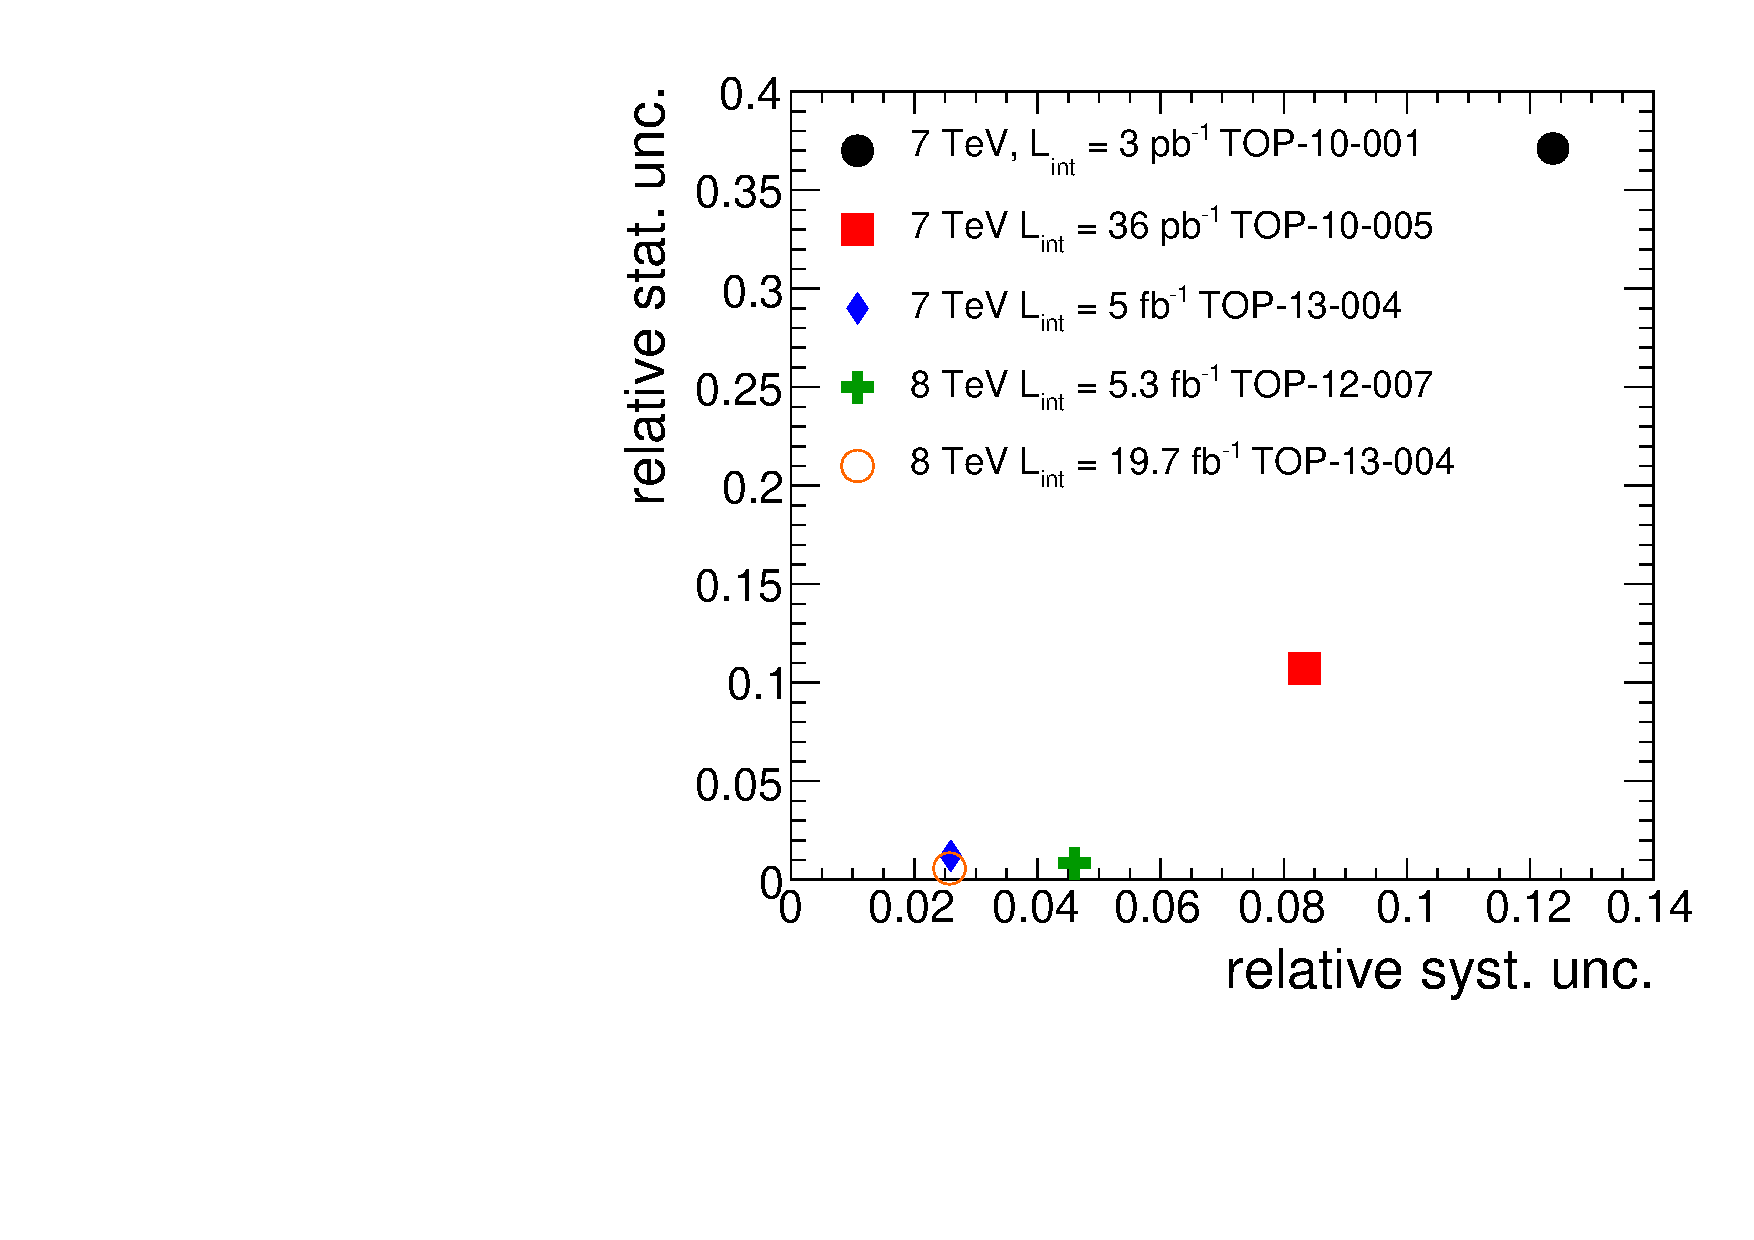
\includegraphics[width= 0.55\textwidth]{figures/top/topToLLXSecUncertaintiesPP.pdf}
  \caption{Evolution of statistical and systematic uncertainty of top pair cross section 
  measurements in the fully leptonic channels in pp collisions at \roots\ = 7 and 8 TeV.
  }
\label{fig:ttStatSyst}
\end{center}
\end{figure}
